\documentclass[twocolumn, 8pt]{extarticle}

% Uncomment to squeeze everything onto one side
%\usepackage{pgfpages}
%\pgfpagesuselayout{2 on 1}[letterpaper, landscape]

\usepackage[letterpaper,margin=0.25in]{geometry}
\input{ncommon}
\everymath{}
\usepackage{titlesec}
\usepackage{multicol}

\usepackage[english]{babel}
\usepackage[autostyle]{csquotes}
\MakeOuterQuote{"}

% Options: [subtle], [moderate], or [extreme]
\usepackage[extreme, mathspacing=normal, lists=normal]{savetrees} 
% Restore space between operators (sin, cos, log) and variables
% \thinmuskip=3mu       % Readable sin/cos
% \medmuskip=2mu        % Tight + and -
% \thickmuskip=3mu      % Tight =
\usepackage{enumitem} % Needs to come after

\titleformat{\section}
  {\normalfont\fontsize{12}{14}\bfseries}{\thesection}{1em}{}
\titlespacing\section{0pt}{5pt plus 2pt minus 2pt}{2pt plus 1pt minus 1pt}
\titlespacing\subsection{0pt}{5pt plus 2pt minus 2pt}{2pt plus 1pt minus 1pt}
\titlespacing\subsubsection{0pt}{5pt plus 2pt minus 2pt}{2pt plus 1pt minus 1pt}
%\renewcommand{\arraystretch}{1.5}
\setlist{nosep}
\setlength{\abovedisplayskip}{3pt}
\setlength{\belowdisplayskip}{3pt}
\setlength{\abovedisplayshortskip}{0pt}
\setlength{\belowdisplayshortskip}{3pt}
\setlength{\parindent}{0pt}
\setlength{\parskip}{2pt}
\raggedbottom
\raggedcolumns

\title{ECE470 Exam Aidsheet}
\author{Tyler Tian}

\begin{document}

\section{Frame Transformations}

\textbf{Points:} \(p^0 = O_0^0 + \rvec{a}{b}{c}^T = O_0 + ax_0^0 + by_0^0 + cz_0^0\)

\textbf{Vectors:} \(v^0 = \rvec{d}{e}{f}^T = dx_0^0 + ey_0^0 + fz_0^0\)

\subsection{Rotations}

\textbf{Rotation Matrices:} \(R_1^0\) denotes the rotation of frame 1 from frame 0.
\[R_1^0 = \rvec{x_1^0}{y_1^0}{z_1^0} = \matthreeb{x_1 \cdot x_0}{y_1 \cdot x_0}{z_1 \cdot x_0}{x_1 \cdot y_0}{y_1 \cdot y_0}{z_1 \cdot y_0}{x_1 \cdot z_0}{y_1 \cdot z_0}{z_1 \cdot z_0}\]
\(R \in SO(3)\) where \(SO(3) = \set{R \in \reals^{3 \times 3} | R^T = R^{-1}, \det(R) = 1}\).

Changing between frames: \(v^0 = R_1^0v^1\). Compose rotations: \(R_2^0 = R_1^0R_2^1\).
\(R_1^0\) is the rotational transformation \(R\) we apply to \(x_0, y_0, z_0\) to get \(x_1, y_1, z_1\).

\textbf{Rotational Transformations:} If \(R\) is expressed in frame 0, then in frame 1, \(R' = (R_1^0)^TR(R_1^0)\).
i.e. \(w^0 = Rv^0 \implies w^1 = R'v^1 = (R_1^0)^TR(R_1^0)v^1\).

When composing rotations each one should be expressed in the new frame after the previous rotation, otherwise a
similarity transformation is needed.

\textbf{Elementary Rotations:}
\[\begingroup
\setlength{\arraycolsep}{2pt}
R_{x, \theta} {=} \matthreeb{1}{0}{0}{0}{\cos\theta}{-\sin\theta}{0}{\sin\theta}{\cos\theta}
\enspace
R_{y, \theta} {=} \matthreeb{\cos\theta}{0}{\sin\theta}{0}{1}{0}{-\sin\theta}{0}{\cos\theta}
\enspace
R_{z, \theta} {=} \matthreeb{\cos\theta}{-\sin\theta}{0}{\sin\theta}{\cos\theta}{0}{0}{0}{1}
\endgroup\]

\textbf{\(zyz\) Euler Angles:} \(R_1^0 = R_{z,\phi}R_{y,\theta}R_{z,\psi} =\)
\[\matthreeb{\cos\phi\cos\theta\cos\psi - \sin\phi\sin\psi}{-\cos\phi\cos\theta\sin\psi - \sin\phi\cos\psi}{\cos\phi\sin\theta}{\sin\phi\cos\theta\cos\psi + \cos\phi\sin\psi}{-\sin\phi\cos\theta\sin\psi + \cos\phi\cos\psi}{\sin\phi\sin\theta}{-\sin\theta\cos\psi}{\sin\theta\sin\psi}{\cos\theta}\]

\begin{minipage}{0.5\linewidth}
    Assuming \(\sin\theta > 0\):
    \begin{align*}
        \theta &= \cos^{-1}(r_{33}) \\
               &= \atantwo\left(\sqrt{1 - r_{33}^2}, r_{33}\right) \\
        \psi &= \atantwo(r_{32}, -r_{31}) \\
        \phi &= \atantwo(r_{23}, r_{13})
    \end{align*}
\end{minipage}
\begin{minipage}{0.5\linewidth}
    Assuming \(\sin\theta < 0\):
    \begin{align*}
        \theta &= -\cos^{-1}(r_{33}) \\
               &= \atantwo\left(-\sqrt{1 - r_{33}^2}, r_{33}\right) \\
        \psi &= \atantwo(-r_{32}, r_{31}) \\
        \phi &= \atantwo(-r_{23}, -r_{13})
    \end{align*}
\end{minipage}

\textbf{Axis-Angle:}
\(\displaystyle\theta = \cos^{-1}\left(\frac{\tr(R) - 1}{2}\right) \qquad
k = \frac{1}{2\sin\theta}\cvec{r_{32} - r_{23}}{r_{13} - r_{31}}{r_{21} - r_{12}}\)

\subsection{Rigid Transformations}

\textbf{Rigid Motions:} \(T(p^0) = Rp^0 + d^0, R \in SO(3), d^0 \in \reals^3 \qquad p^0 = O_1^0 + R_1^0p^1\)

\textbf{Homogeneous Transformations:} \(P^0 = \cvec{p^0}{1} = H_1^0\cvec{p^1}{1}, H_1^0 \in SE(3)\)
\[SE(3) = \Set{\mattwo{R}{d}{0_{1 \times 3}}{1} | R \in SO(3), d \in \reals^3} \qquad H^{-1} = \mattwo{R^T}{-R^Td}{0_{1 \times 3}}{1}\]
\(\Rot_{x,\alpha}\) denotes pure rotation, \(\Trans_{x,a}\) denotes pure translation.

\subsection{Velocity Transformations}

\textbf{Skew-Symmetric Form:}
\begin{gather*}
S(w) = \matthree{0}{-w_z}{w_y}{w_z}{0}{-w_x}{-w_y}{w_x}{0} \qquad w \times v = S(w)v \qquad x^TS(w)x = 0 \\
S(w_1 + \lambda w_2) = S(w_1) + \lambda S(w_2) \qquad RS(w)R^T = S(Rw),\forall R \in SO(3)
\end{gather*}

\textbf{Cross Product:} \(a \times b = -b \times a \quad R(a \times b) = (Ra) \times (Rb), \forall R \in SO(3)\)

\textbf{Angular Velocity:} \(\dot R_1^0 = S(w_1^0)R_1^0 \iff S(w_1^0) = \dot R_1^0(R_1^0)^T\) where \(w_1^0\) is the angular velocity of frame 1 with
respect to frame 0 (expressed in frame 0).
Compose through addition: \(w_2^0 = w_1^0 + R_1^0w_2^1\).

Shorthand: \(w_{i,j}^k = R_i^kw_j^i \qquad w_n^0 = w_{0,1}^0 + \cdots + w_{n - 1, n}^0 = \sum _{i = 1}^n R_{i - 1}^0w_i^{i - 1}\)

Linear velocity of a point on a rotating body is \(v = w \times p\) where \(p\) is a vector from the axis of rotation.

\textbf{Velocity in Another Frame:} For point \(p\) with velocity \(\dot p^1\) and position \(p^1\) in frame 1, moving
relative to 0, \(\dot p^0 = \dot O_1^0 + w_1^0 \times (R_1^0p^1) + R_1^0\dot p^1\).

For frames, \(\dot O_2^0 = \dot O_1^0 + w_1^0 \times (R_1^0O_2^1) + R_1^0\dot O_2^1\).

\section{Denavit-Hartenberg Parameters}

\textbf{DH Frame Rules:} Frame 0 is the inertial frame; frame \(i\) is rigidly attached to link \(i\), so when joint
\(i\) is actuated, frame \(i\) moves with link \(i\). Axis rules: \(x_i\) is orthogonal to and intersects \(z_{i - 1}\).

\textbf{DH Frame Assignment:}
\begin{enumerate}
    \item Assign \(z_i\) to the axis of actuation of joint \(i + 1\) and assign \(x_0\) arbitrarily.
    \item Assign \(x_i\) for \(i = 1, \dots, n - 1\) according to cases:
    \begin{enumerate}
        \item \(z_{i - 1}\), \(z_i\) not coplanar: \(x_i\) is in the direction of the shortest segment joining the axes.
        \item \(z_{i - 1}\), \(z_i\) intersect: \(x_i\) is normal to the plane formed by \(z_{i - 1}\), \(z_i\).
        \item \(z_{i - 1}\), \(z_i\) parallel: \(x_i\) is any vector orthogonal and intersecting \(z_{i - 1}\).
    \end{enumerate}
    \item Assign the end-effector \(x_n\) orthogonal and intersecting \(z_{i - 1}\), then \(z_n\) arbitrarily.
\end{enumerate}

\begin{center}
    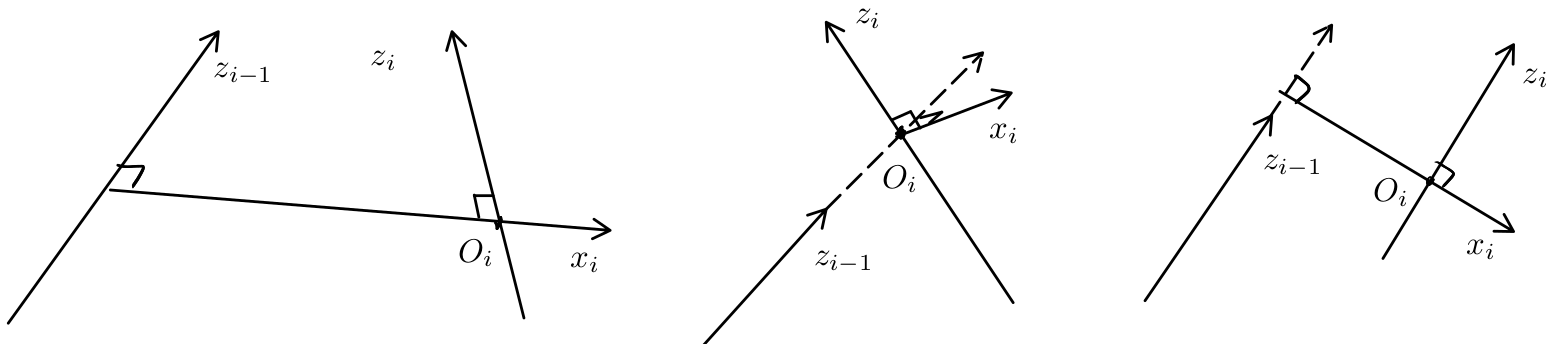
\includegraphics[width=\linewidth]{imgs/dh_cases.png}
\end{center}
\vspace{-1em}

\textbf{DH Parameters:}
\begin{enumerate}
	\item Link length $a_i$: the signed distance between $z_{i - 1}$ and $z_i$, along $x_i$
    \item Link twist $\alpha _i$: the signed angle between $z_{i - 1}$ and $z_i$, about $x_i$
	\item Link offset $d_i$: the signed distance between $O_{i - 1}$ and $O_i$, along $z_{i - 1}$
	\item Joint angle $\theta _i$: the signed angle between $x_{i - 1}$ and $x_i$, about $z_{i - 1}$
\end{enumerate}

\vspace{-1em}
\begin{center}
    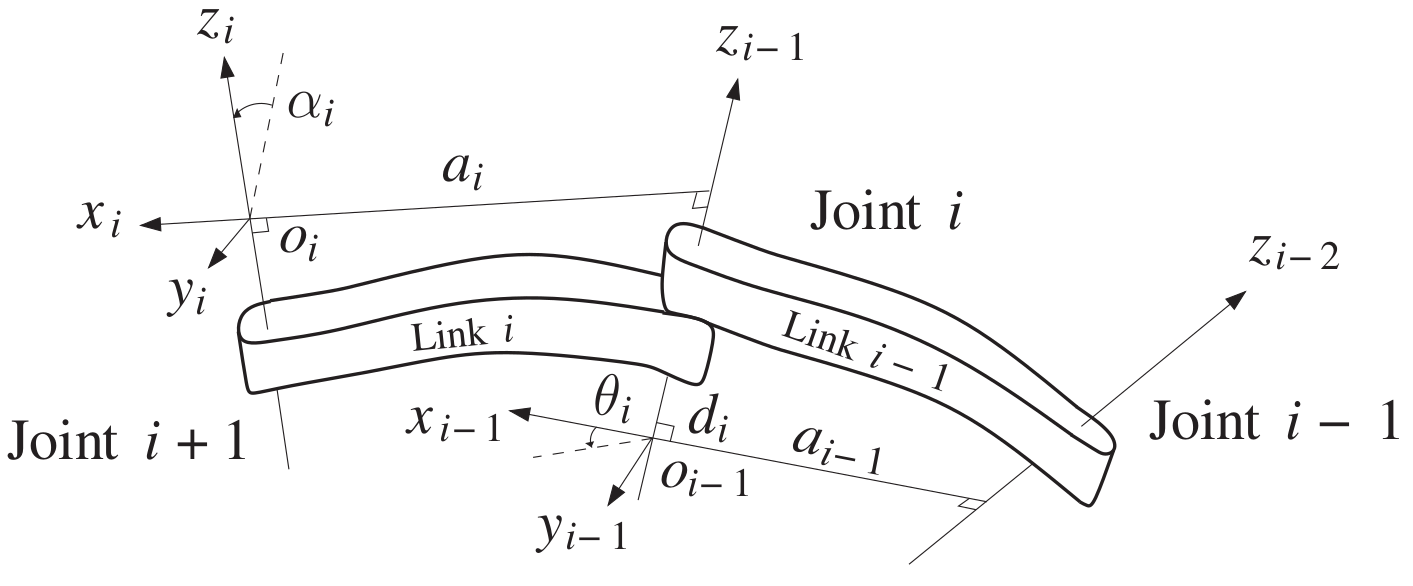
\includegraphics[width=0.8\linewidth]{imgs/dh.png}
\end{center}
\vspace{-1.5em}

\textbf{DH Homo. Transform:} \(H_i^{i - 1} = \Rot_{z, \theta _i}\Trans_{z, d_i}\Trans_{x, a_i}\Rot_{x, \alpha _i}\)
\[
\matfour{\cos\theta _i}{-\sin\theta _i\cos\alpha _i}{\sin\theta _i\sin\alpha _i}{a_i\cos\theta _i}{\sin\theta _i}{\cos\theta _i\cos\alpha _i}{-\cos\theta _i\sin\alpha _i}{a_i\sin\theta _i}{0}{\sin\alpha _i}{\cos\alpha _i}{d_i}{0}{0}{0}{1}
\]

\textbf{Recovering Manipulator From DH Table:}
\begin{enumerate}
	\item Start at frame 0 and move to next frame in sequence.
	\item Identify direction of \(x_{i + 1}\) by rotating \(x_i\) by \(\theta _i\) around \(z_i\).
	\item Identify \(O_{i + 1}\) by moving \(d_i\) along \(z_i\) and \(a_i\) along \(x_{i + 1}\).
	\item Identify direction of \(z_{i + 1}\) by rotating \(\alpha _i\) along \(x_{i + 1}\).
\end{enumerate}

\section{Kinematics}

\subsection{Forward Kinematics}

Given joint angles \(q\), \(H_n^0(q) = H_1^0(q_1)H_2^1(q_2)\cdots H_n^{n - 1}(q_n)\).

\subsection{Inverse Kinematics}

If \(n < 6\), no solutions in general. If \(n = 6\) there are finite solutions. If \(n > 6\) there are infinite
solutions.

\textbf{Kinematic Decoupling:} Assuming \(n = 6\) and last 3 joints form a spherical wrist, \(x_4 = -z_3 \times z_4\).
Let \(O_c^0 = O_d^0 - R_d^0\rvec{a_6}{0}{d_6}^T\). Solve for \(q_1, q_2, q_3\) given desired \(O_c = O_4 = O_5\).
Then using \(R_6^3 = (R_3^0)^TR_d^0\) solve for \(q_4, q_5, q_6\) as \(zyz\) Euler angles
(\(q_4 = \phi, q_5 = \theta, q_6 = \psi\)).

\begin{minipage}{0.4\linewidth}
    \begin{center}
        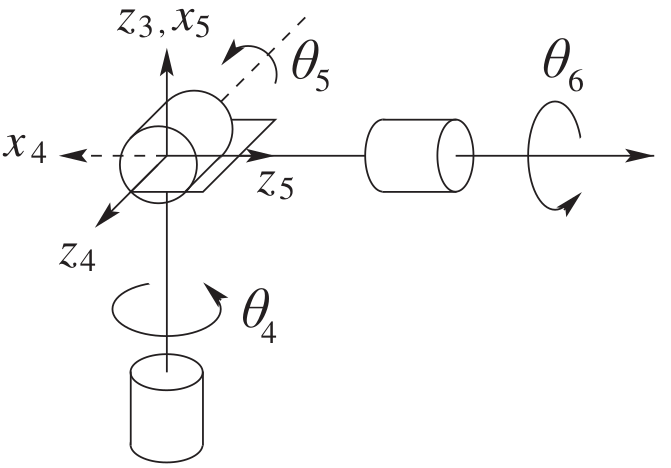
\includegraphics[width=\linewidth]{imgs/spherical_wrist_cropped.png}
    \end{center}
\end{minipage}%
\hfill%
\begin{minipage}{0.5\linewidth}
    \textbf{Spherical Wrist DH Table:}
    \begin{center}
        \begin{tabular}{c | c c c c}
            Link & \(a\) & \(\alpha\) & \(d\) & \(\theta\) \\
            \hline
            4 & 0 & \(-\pi/2\) & \(d_4\) & \(\theta _4^*\) \\
            5 & 0 & \(\pi/2\) & \(0\) & \(\theta _5^*\) \\
            6 & \(a_6\) & \(0\) & \(d_6\) & \(\theta _6^*\) \\
        \end{tabular}
    \end{center}
\end{minipage}

\subsection{Forward Velocity Kinematics}

\textbf{End-Effector Velocity:} \(\dot O_i^0 = \dot O_{i - 1}^0 + w_{i - 1}^0 \times (R_{i - 1}^0O_i^{i - 1}) + R_{i - 1}^0\dot O_i^{i - 1}\)
where \(O_i^0 = O_{i - 1}^0 + R_{i - 1}^0O_i^{i - 1}, w_i^0 = w_{i - 1}^0 + R_{i - 1}^0w_i^{i - 1}\).

Revolute joint: \(w_i^{i - 1} = \rvec{0}{0}{\dot q_i}^T, \dot O_i^{i - 1} = w_i^{i - 1} \times O_i^{i - 1}\).

Prismatic joint: \(w_i^{i - 1} = 0, \dot O_i^{i - 1} = \rvec{0}{0}{\dot q_i}^T\)

\textbf{Strategy:} If forward kinematic expression is simple, get \(\dot O_n^0\) by direct differentiation, and get
\(w_n^0\) by \(S(w_n^0) = \dot R_n^0(R_n^0)^T\) and directly differentiating the rotation matrix. Use Jacobian formulas
otherwise.

\textbf{Indicator Function:} \(\rho _i = 0\) for prismatic joints, 1 for revolute joints.

\textbf{Angular Velocity Jacobian:} \(w_n^0 = J_w(q)\dot q, J_w(q) = \pdiff{w_n(q)}{q} \in \reals^{3 \times n}\)
\[J_w(q) = \rvec{\rho _1 z_0^0}{\rho _2 z_1^0}{\cdots}{\rho _n z_{n - 1}^0}\]

\textbf{Linear Velocity Jacobian:} \(\dot O_n^0 = J_v(q)\dot q, J_v(q) = \pdiff{O_n^0(q)}{q} \in \reals^{3 \times n}\)
\[J_v(q) = \rvec{J_{v,1}(q)}{\cdots}, J_{v,i}(q) = \twocond{z_{i - 1}^0}{i\text{ prismatic}}{z_{i - 1}^0 \times (O_n^0 - O_{i - 1}^0)}{i\text{ revolute}}\]

The complete Jacobian is \(J(q) = \cvec{J_v(q)}{J_w(q)}\).

\subsection{Inverse Velocity Kinematics}

If \(n < 6\), no solutions in general. If \(n = 6\), (unique) solution exists iff \(J(q)\) is invertible. If \(n > 6\),
infinite solutions exist, iff \(J(q)\) has rank 6.

\textbf{Pseudoinverse:} \(J^\dagger = J^T(JJ^T)^{-1}\), satisfies \(JJ^\dagger = I\).

\textbf{\(n > 6\) Solution:} \(\dot q = J^\dagger(q)\xi + (I - J^\dagger(q)J(q))b\) where \(b \in \reals^n\) is
arbitrary and \(\xi = (\dot O_n^0, w_n^0)\) is the desired velocity.

\section{Other Applications}

\textbf{Basic Motion Planning:} Define quadratic potential \(U(q) = \frac{1}{2}\norm{O_d^0 - O_n^0(q)}^2\).
Use velocity
\(\displaystyle \dot q = -\gamma\nabla _q\mathcal U(q) = \gamma\left(\pdiff{O_n^0(q)}{q}\right)^T(O_d^0 - O_n^0(q))\).

\textbf{Numerical Inverse Kinematics:} Let \(x = \rvec{(O_n^0)^T}{\phi}{\theta}{\psi}^T \in \reals^6\) describe the state (end-effector pose).
The analytic Jacobian \(J_a(q)\) contains derivatives of \(x\) with respect to \(q\), and satisfies
\(\dot x = J_a(q)\dot q, \dot q = J_a^\dagger(q)\dot x\).
Form ODE \(\dot q = J_a^\dagger(q)K(x_d - x(q)) = J_a^\dagger(q)Ke\) and solve using numerical methods, and \(q\) should
converge to a solution.

\textbf{End-Effector Force and Torque:}
Given desired wrench at the end-effector \(F^0 = \rvec{f^0}{n^0}^T\) where \(f^0\) is a force and \(n^0\) is a torque,
each joint's force/torque is \(\tau = J^T(q)F^0\).

\subsection{Potential Field Path Planning}

\textbf{Potential Field Method:} Given \(q^s, q^f\), convex obstacles, initialize \(q^0 = q^s\),
\[q^{k + 1} = q^k + \alpha _k\sum _{i = 1}^n J_{v,O_i}^T(q^k)\left(F_{i,att}(O_i^0(q^k)) + F_{i,rep}(O_i^0(q^k))\right)\]
until convergence \(\norm{q^{k + 1} - q^f} < \varepsilon\), outputs a set of waypoints in joint space.

\textbf{Attractive Potential:} $\displaystyle \mathcal U_{i, att}(O_i^0) = \frac{1}{2}c_i\norm{O_i^0 - \bar O_i^0}^2$ for weights
$c_i > 0$. Gradient: \(\displaystyle F_{i, att}(O_i^0) = -\nabla \mathcal U_{i, att}(O_i^0) = -c_i(O_i^0 - \bar O_i^0)\).

\textbf{Repulsive Potential:} For weights \(\eta_i > 0\), region of influence \(\rho _0\), and closest obstacle point
\(\pi(O_i^0)\), when \(\rho(O_i^0) = \norm{O_i^0 - \pi(O_i^0)} > \rho _0\):
\[\mathcal U_{i, rep} = \frac{\eta _i}{2}\left(\frac{1}{\rho(O_i^0)} - \frac{1}{\rho _0}\right)^2
\quad F_{i,rep}(O_i^0) = \eta _i\left(\frac{1}{\rho(O_i^0)} - \frac{1}{\rho _0}\right)\frac{(O_i^0 - \pi(O_i^0))}{\rho(O_i^0)^3}\]

\textbf{Jacobians:} \(J_{v,O_i}(q) = \pdiff{O_i^0(q)}{q} = \rvec{J_{v,O_i,1}}{\cdots}{J_{v,O_i,i}}{0_{3 \times (n - i)}}\)
where \(J_{v,O_i,j} = z_{j - 1}^0 \times (O_i^0 - O_{j - 1}^0)\) for revolute, \(J_{v,O_i,j} = z_{j - 1}^0\) for prismatic.

\textbf{Spline Interpolation:} Find $q: \reals \mapsto \reals^n \in \mathcal C^2$ such that $q(0) = q^0$ and $q(t_i) = q_i$.
Each segment is \(P_i(t) = a_3^it^3 + a_2^it^2 + a_1^it + a_0^i, t \in [t_i, t_{i + 1}]\) for \(i = 0, \dots, N - 1\),
total \(4N\) unknowns in \(\reals^n\), with constraints:
\begin{enumerate}
    \item Interpolation: \(P_i(t_i) = q^i\) for \(i = 0, 1, \dots, N - 1\) and \(P_{N - 1}(t_N) = q^N\).
    \item Twice-differentiability: \(P_i(t_{i + 1}) = P_{i + 1}(t_{i + 1})\), \(\dot P_i(t_{i + 1}) = \dot P_{i + 1}(t_{i + 1})\), \(\ddot P_i(t_{i + 1}) = \ddot P_{i + 1}(t_{i + 1})\) for \(i = 0, 1, \dots, N - 2\).
    \item Endpoint acceleration: \(\ddot P_0(t_0) = \ddot P_{N - 1}(t_N) = 0\).
\end{enumerate}

\section{Robot Modelling}

\textbf{Euler-Lagrange:} For Lagrangian \(\mathcal L = T - \mathcal U\), \(n\) degrees of freedom ($n = 3N - l$ for $l$
constraints and $N$ particles in 3 dimensions), generalized coordinates \(q\):

\(\displaystyle\diff{}{t}\left(\pdiff{\mathcal L}{\dot q_j}\right) - \pdiff{\mathcal L}{q_j} = \tau _j\)
where \(\displaystyle \tau _j = \sum _{i = 1}^N (f_i^l)^T\pdiff{r_i}{q_j}\)
for applied forces $f^l$.

\textbf{Holonomic Constraints:} Expressed as \(g(r_1, \dots, r_N) = 0 \in \reals^l\), assuming independence:
\(\rank\left(\pdiff{g}{r}\right) = l\).

\textbf{Virtual Displacements:}
\(\delta r = \rvec{\delta r_1^T}{\cdots}{\delta r_N^T}^T \in \reals^{3N}\)
must satisfy \(\pdiff{g}{r}\delta r = 0\).
All possible virtual displacements are described by \(\delta r = \pdiff{r}{q}\dd q\).

\textbf{Canonical Robot Model:} \(D(q)\ddot q + C(q, \dot q)\dot q + G(q) = \tau\) where:
\begin{enumerate}
	\item $D(q) = \sum _{i = 1}^n \left[m_iJ_{v_i}^T(q)J_{v_i}(q) + J_{w_i}^T(q)R_i^0\bar I_i(R_i^0)^TJ_{w_i}^T(q)\right]$
	\item $\left[C(q, \dot q)\right]_{kj} = \sum _{i = 1}^n c_{ijk}(q)\dot q_i$ where $\displaystyle c_{ijk} = \frac{1}{2}\left(\pdiff{d_{kj}}{q_i} + \pdiff{d_{ki}}{q_j} - \pdiff{d_{ij}}{q_k}\right)$
	\item $G(q) = \nabla _q\mathcal U(q)$ where $\mathcal U(q) = -\sum _{i = 1}^n m_i\bar g^Tr_i^0(q)$ is the potential energy.
\end{enumerate}
for body-fixed inertias $\bar I_i$, COMs $r_i^0$, gravity $\bar g = \rvec{0}{0}{-g}^T$.
For non-constant inertias transform as \(I_i = R_i^0\bar I_i(R_i^0)^T\).

\textbf{Kinetic Energy:} \(\displaystyle T = \sum _{i = 1}^N \frac{1}{2}m_i\norm{\dot r_i}^2 + \frac{1}{2}(w_i^0)^TR_i^0\bar I_i(R_i^0)^Tw_i^0 = \frac{1}{2}\dot q^TD(q)\dot q\)

\textbf{Partial Jacobians:}
\begin{align*}
J_{v_i} &= \twocond{\rvec{z_0^0 \times (r_i^0 - O_0^0)}{\cdots}{z_{i - 1}^0 \times (r_i^0 - O_{i - 1}^0)}{0_{3 \times (n - i)}}}{\text{revolute}}{\rvec{z_0^0}{z_1^0}{\cdots}{z_{i - 1}^0}{0_{3 \times (n - i)}}}{\text{prismatic}} \\
J_{w_i} &= \rvec{\rho _1z_0^0}{\rho _2z_1^0}{\cdots}{\rho _iz_{i - 1}^0}{0_{3 \times (n - i)}}
\end{align*}

\section{Lyapunov Theory}

Consider general nonlinear systems \(\dot x = f(x), x \in \reals^n, f: \reals^n \mapsto \reals^n \in \mathcal C^1\), with
equilibria \(\bar x \in \reals^n\) where \(f(\bar x) = 0\).

\textbf{Lyapunov Stability:} \(\forall \varepsilon > 0, \exists \delta > 0 \suchthat \norm{x(0)} < \delta \implies
\norm{x(t)} < \varepsilon, \forall t \geq 0\), i.e. we can stay arbitrarily close to the equilibrium forever by starting close
enough to the equilibrium.

\textbf{Asymptotic Stability:} Stable and \(\displaystyle\exists \delta _0 > 0 \suchthat \norm{x(0)} < \delta _0 \implies \lim _{t \to \infty} x(t) = 0\),
i.e. solutions converge to the equilibrium within some radius.

\textbf{Definiteness:} \(U: \reals^n \mapsto \reals\) is positive definite at \(x = 0\) if \(U(0) = 0\) and \(x \neq 0
\implies U(x) > 0\); positive semidefinite if \(U(x) = 0\) and \(U(x) \geq 0, \forall x\).

\textbf{Lyapunov's Theorem:} If there exists a Lyapunov function \(V: \reals^n \mapsto \reals \in \mathcal C^1\) which
is positive definite at \(\bar x\), then if $\dot V(x) = \pdiff{V}{x}f(x)$ is negative semidefinite,
\(\bar x\) is stable. If $\dot V(x)$ is negative definite, then \(\bar x\) is asymptotically stable.

\textbf{LaSalle Invariance Principle}: If \(V\) is positive definite at \(\bar x\), and \(\displaystyle \dot V(x) =
\pdiff{V}{x}f(x) \leq 0\), then \(\displaystyle \lim _{t \to \infty} \dot V(x(t)) = 0\). If $\dot V(x) \equiv 0, \forall
t \implies x(t) \equiv \bar x, \forall t$, i.e. the only way to have \(\dot V = 0\) for all time is to be at the
equilibrium, then \(\bar x\) is asymptotically stable.

\section{Robot Control}

\textbf{Simplified Motor Model:} \(J\ddot\theta _m + B\dot\theta _m = u - \tau _l\) for voltage \(u\), load \(\tau _l\).

\textbf{Augmented Robot Model:} \(M(q)\ddot q + C(q, \dot q)\dot q + B(q)\dot q + G(q) = u\) for motor voltages \(u\),
back-EMF \(B(q)\) (positive definite), \(M(q) = D(q) + J\) where \(J = \diag\set{J_{m_i}}\).
Note \(\dot M(q, \dot q) - 2C(q, \dot q)\) is skew-symmetric.

\textbf{Decentralized (Independent Joint) Control:} \(u = J\ddot q^r + B\dot q^r + K_pe + K_d\dot e\) for \(K_p, K_d >
0\), where \(e(t) = q^r(t) - q(t)\), assuming each \(\theta _m = q \in \reals\).
Each joint has dynamics \(\ddot e + \frac{B}{J}\dot e = \ddot q^r + \frac{B}{J}\dot q^r - \frac{1}{J}u\), closed-loop
dynamics \(\ddot e + \left(\frac{B}{J} + \frac{K_D}{J}\right)\dot e + \frac{K_p}{J}e = 0\).
Treats robot dynamics as disturbances.

\textbf{Feedback Linearization:} \(u = M(q)v + C(q, \dot q)\dot q + B(q)\dot q + G(q)\) where
\(v = \ddot q^r + K_p\tilde q + K_d\dot{\tilde q}\), for error \(\tilde q = q^r - q\) and diagonal, positive definite
\(K_p, K_d\). Closed-loop dynamics \(\ddot q = v \iff \ddot{\tilde q} + K_d\dot{\tilde q} + K_p\tilde q = 0\).
This requires perfect knowledge of system parameters so does not work well in practice.

\textbf{PD Control With Gravity Compensation:} \(u = K_p\tilde q + K_d\dot{\tilde q} + G(q)\) where \(\tilde q = q^r - q\)
and reference \(q^r\) is constant, for positive definite \(K_p, K_d\).
Closed-loop dynamics \(M(q)\ddot q + C(q, \dot q)\dot q + B(q)\dot q = K_p\tilde q + K_d\dot{\tilde q}\).
Lyapunov function
\( V(q, \dot q) = \frac{1}{2}\dot q^TM(q)\dot q + \frac{1}{2}(q - q^r)^TK_p(q - q^r) \implies \dot V = -\dot q^T(B(q) + K_d)\dot q\).
Can only track a constant reference but only requires knowledge of gravity terms.

\textbf{Passivity-Based Control:} Define \(r = \dot{\tilde q} + \Lambda\tilde q\) where \(\tilde q = q^r - q\) and
\(\Lambda\) diagonal,
\(u = M(q)(\ddot q^r + \Lambda\dot{\tilde q}) + C(q, \dot q)(\dot q^r + \Lambda\tilde q) + B(q)\dot q + G(q) + K(\dot{\tilde q} + \Lambda\tilde q)\)
with closed-loop dynamics \(M(q)\dot r + (C(q, \dot q) + K)r = 0\).
Use Lyapunov function \( V = \frac{1}{2}r^TM(q)r + \tilde q^T\Lambda K\tilde q \implies \dot V = -\dot{\tilde q}^TK\dot{\tilde q} - \tilde q^T\Lambda K\Lambda\tilde q\).

\textbf{Linear Parametrization:} \(M(q)\ddot q + C(q, \dot q)\dot q + B(q)\dot q + G(q) = Y(q, \dot q, \ddot q)\Phi\)
where \(Y(q, \dot q, \ddot q)\) is a known regressor matrix for the structure of the robot, and \(\Phi\) is an unknown
vector containing all the physical parameters of the robot.

\textbf{Adaptive Passivity-Based Control:} \(u = -Kr + Y\hat\Theta\) where \(r =
\dot{\tilde q} + \Lambda\tilde q, v = \dot q^r - \Lambda\tilde q, a = \ddot q^r - \Lambda\dot{\tilde q} = \dot v\), with
error \(\tilde q = q - q^r\) (reversed!), for positive definite \(K, \Lambda, \Gamma\), regressor \(Y\) such that
\(M(q)a + C(q, \dot q)v + B(q)\dot q + G(q) = Y(q, \dot q, a, v)\Theta\), and parameter estimate \(\hat\Theta\), with
adaptation law \(\dot{\hat\Theta} = -\Gamma Y^Tr\) for learning rate \(\Gamma\).

Closed-loop dynamics \(M(q)\dot r + (C(q, \dot q) + K)r = Y(q, \dot q, a, v)\tilde\Theta\) (substitute using
\(\dot q = r + v, \ddot q = \dot r + a\)) where \(\tilde\Theta = \hat\Theta - \Theta\).
Use Lyapunov function \( V = \frac{1}{2}r^TM(q)r + \tilde q^T\Lambda K\tilde q + \frac{1}{2}\tilde\Theta^T\Gamma^{-1}\tilde\Theta
\implies \dot V = -\dot{\tilde q}^TK\dot{\tilde q} - \tilde q^T\Lambda K\Lambda\tilde q\).

This tracks the reference but does not guarantee asymptotic convergence of \(\hat\Theta\), which requires a persistence
of excitation condition. This controller does not require knowledge of system parameters but results in aggressive
transient behaviour.

\section{Useful Identities}

\begin{gather*}
    {\textstyle\sin\left(x + \frac{\pi}{2}\right) = \cos(x) \quad \sin\left(x - \frac{\pi}{2}\right) = -\cos(x) \quad \sin\left(\frac{3\pi}{2} - x\right) = -\cos(x)} \\
    {\textstyle\cos\left(x + \frac{\pi}{2}\right) = -\sin(x) \quad \cos\left(x - \frac{\pi}{2}\right) = \sin(x) \quad \cos\left(\frac{3\pi}{2} - x\right) = \sin(x)} \\
    \sin(x + y) = \sin x\cos y + \cos x\sin y \quad \sin(x - y) = \sin x\cos y - \cos x\sin y \\
    \cos(x + y) = \cos x\cos y - \sin x\sin y \quad \cos(x - y) = \cos x\cos y + \sin x\sin y \\
    \atantwo(-y, x) = -\atantwo(y, x) \qquad \atantwo(y, -x) = \pi - \atantwo(y, x) \\
    \forall a > 0,\,\atantwo(ay, ax) = \atantwo(y, x) \\
    \atantwo\left(x, \sqrt{1 - x^2}\right) = \sin^{-1} x \qquad \atantwo\left(\pm\sqrt{1 - x^2}, x\right) = \pm\cos^{-1} x \\
    \atantwo\left(x, -\sqrt{1 - x^2}\right) = \twocond{\pi - \sin^{-1}x}{x > 0}{-\pi - \sin^{-1}(x)}{x < 0} \\
    \nabla _x f(x) = \left(\pdiff{f(x)}{x}\right)^T \qquad \pdiff{\norm{x}}{x} = \frac{1}{\norm{x}}x^T \\
    v_1 \cdot v_2 = \norm{v_1}\norm{v_2}\cos\theta \qquad v_1 \times v_2 = \norm{v_1}\norm{v_2}\sin(\theta)\hat n
\end{gather*}

\end{document}
